% THIS IS SIGPROC-SP.TEX - VERSION 3.1
% WORKS WITH V3.2SP OF ACM_PROC_ARTICLE-SP.CLS
% APRIL 2009
%
% It is an example file showing how to use the 'acm_proc_article-sp.cls' V3.2SP
% LaTeX2e document class file for Conference Proceedings submissions.
% ----------------------------------------------------------------------------------------------------------------
% This .tex file (and associated .cls V3.2SP) *DOES NOT* produce:
%       1) The Permission Statement
%       2) The Conference (location) Info information
%       3) The Copyright Line with ACM data
%       4) Page numbering
% ---------------------------------------------------------------------------------------------------------------
% It is an example which *does* use the .bib file (from which the .bbl file
% is produced).
% REMEMBER HOWEVER: After having produced the .bbl file,
% and prior to final submission,
% you need to 'insert'  your .bbl file into your source .tex file so as to provide
% ONE 'self-contained' source file.
%
% Questions regarding SIGS should be sent to
% Adrienne Griscti ---> griscti@acm.org
%
% Questions/suggestions regarding the guidelines, .tex and .cls files, etc. to
% Gerald Murray ---> murray@hq.acm.org
%
% For tracking purposes - this is V3.1SP - APRIL 2009

\documentclass{acm_proc_article-sp}

\usepackage{amsmath}
\usepackage{algorithm}
\usepackage[noend]{algpseudocode}
\begin{document}

\title{toMEto: a Networks-based Approach to Recipe Recommendation}
\subtitle{CS145}


\makeatletter
\def\BState{\State\hskip-\ALG@thistlm}
\makeatother


\numberofauthors{4} 
\author{
\alignauthor
Albert Ge\\
       \affaddr{California Institute of Technology}\\
       \affaddr{Pasadena, CA}\\
       \email{age@caltech.edu}
\alignauthor
Matthew Jin\\
       \affaddr{California Institute of Technology}\\
       \affaddr{Pasadena, CA}\\
       \email{mjin@caltech.edu}
\and % go to new row
\alignauthor
Jonathan Joo\\
       \affaddr{California Institute of Technology}\\
       \affaddr{Pasadena, CA}\\
       \email{jjoo@caltech.edu}
\alignauthor
Boyu (Charlie) Tong\\
       \affaddr{California Institute of Technology}\\
       \affaddr{Pasadena, CA}\\
       \email{bttong@caltech.edu}
}

\date{20 April 2013}


\maketitle
\begin{abstract}
Abstract text. Abstract text. Abstract text. Abstract text. Abstract text. Abstract text. Abstract text. 
\end{abstract}

% A category with the (minimum) three required fields
%\category{H.4}{Information Systems Applications}{Miscellaneous}
%A category including the fourth, optional field follows...
%\category{D.2.8}{Software Engineering}{Metrics}[complexity measures, performance measures]

%\terms{Theory}

%\keywords{ACM proceedings, \LaTeX, text tagging} % NOT required for Proceedings

\section{Introduction}
Cooking is a 

\section{Related Work}

There have been a select number of papers discussing analysis of food and ingredient networks. Teng et al. describes the goal of being able to recommend entire recipes, using recipe suggestions made by examining communities of a co-occurrence network, to predict the success of a particular recipe's rating ~\cite{recommend}. 

Another paper by Ahn et al. compares the differences in cuisine by instead looking at a flavor-compounds network, and making general statements about the co-occurrence of ingredients by their chemical composition ~\cite{pairings}. They discovered that Asian recipes tend to have ingredients with different compounds, whereas Western cuisines have ingredients with like compounds. 

Still other research is ongoing, some building upon the relevance of flavor compounds 
in regional cuisines ~\cite{zhu2013geography}, ~\cite{jain2015analysis}, and others attempt to implement these ideas to help users make suggestions about healthy food choices ~\cite{Geleijnse}.

Within this web of research, we discovered a potential niche for recommending individual \textit{ingredients}, as opposed to entire recipes. This combines both the practical application of current research on food networks, as well as the theory behind identifying ingredients thaFigure~\ref{fig:}t are compatible with each other.


\section{Data Processing}

\subsection{Data source}
Our application's source of data are the online recipe websites New York Times (NYT) Cooking and AllRecipes.com. We gained over 13,000 and 52,000 recipes by crawling and scraping these two websites respectively. This was done by a script written in \texttt{scraper.py}. 

\subsection{Initial parsing}
Our application only requires the title, ingredients, and body of each recipe, so we extracted this data from each webpage using a simple script written in \texttt{parser.py}.

However, this extracted data was not in a clean format that our algorithms could easily use. For example, ingredients were often combined with quantifiers and other adjectives:
\begin{itemize}
       \item {\em medium-size russet potato, about 10 ounces, peeled and diced}
       \item {\em shrimp, shelled and cut into bite-sized pieces}
       \item {\em kale, stemmed, rinsed and coarsely chopped to make 6 cups}
\end{itemize}
These ingredients would only occur maybe once or twice in the entire dataset, resulting in many ``rare'' ingredients. In the NYT dataset (12402 unique ingredients), approximately 70\% of the unique ingredients occurred only once, and 90\% occurred less than 10 times. We realized this resulted in suboptimal performance, as these ingredients would not be counted correctly in the co-occurrence network and many edges would not exist in the network.

\subsection{Mapping}
To fix this, we developed a script in \texttt{nyt\_mapper.py} to find these ``rare'' ingredients and map them to their root ingredient. For the example ingredients from above, we generated the mappings:
\begin{itemize}
       \item {\em medium-size russet potato, about 10 ounces, peeled and diced} $\to$ {\em potato}
       \item {\em shrimp, shelled and cut into bite-sized pieces} $\to$ {\em shrimps}
       \item {\em kale, stemmed, rinsed and coarsely chopped to make 6 cups} $\to$ {\em kale}
\end{itemize}
The script attempts to extract the root ingredient for each entry by combining several strategies. For example, some strategies that we use are:
\begin{itemize}
       \item Removing parenthetical tokens 
       \begin{itemize}
              \item {\em vanilla extract (to taste)} $\to$ {\em vanilla extract}
       \end{itemize}
       \item Removing comma separated descriptors 
       \begin{itemize}
              \item {\em honey, preferably wildflower} $\to$ {\em honey}
       \end{itemize}
       \item Picking the best of two ingredients separated by `or' 
       \begin{itemize}
              \item {\em sriracha or other hot sauce} $\to$ {\em sriracha}
       \end{itemize}
       \item Finding a sole `top' ingredient name 
       \begin{itemize}
              \item {\em coarsely grated carrot} $\to$ {\em carrots}
       \end{itemize}
\end{itemize}
Using the mappings generated by \texttt{nyt\_mapper.py}, we reduced the unique ingredient count by 75\%. This resulted in a much more densely connected network, and more accuracy in recommendations.

\subsection{Supplementing with AllRecipes data}
We initially focused our application on the NYT dataset due to the relatively cleaner data and ingredients list. Once our basic algorithms were up and running on this dataset, we moved to supplement it with the much larger AllRecipes dataset. We reasoned that this would further improve the co-occurrence network by providing a more accurate count of ingredient frequencies. We also realized it would introduce new connections, since there may be recipes and foods that are not found in the NYT dataset.

As our application does recommendations only for NYT recipes, we modified our approach to processing the AllRecipes data accordingly. Again, we wrote a mapping script in \texttt{allrecipes\_mapper.py}, but instead of mapping to only the root ingredients, the script also attempted to map to the top ingredients in the NYT dataset. This was important because our goal ultimately was to develop a co-occurrence network for the NYT dataset, and we did not want the ingredients of the AllRecipes dataset to be disjoint in any way. 

The AllRecipes mapper employed many of the same techniques as the NYT mapper, with some additional strategies. The recipes from the AllRecipes websites list the ingredients with numbers and quantifiers, for example:
\begin{itemize}
       \item {\em 1 pound ground beef}
       \item {\em 1/2 teaspoon black pepper}
       \item {\em 1 (25 ounce) package frozen cheese ravioli}
\end{itemize}
Thus, we added filters that removed numerical digits from the raw ingredient name and also searched for and removed quantifiers such as ``pound'', ``teaspoon'', or ``ounce''. To map the ingredients to the NYT ingredients, we took a set of the most common NYT ingredients and searched for corresponding tokens in the AllRecipes ingredients. If there was a 1-to-1 matching, then we considered it a mapping.

Combining both datasets resulted in a network with 7339 unique ingredients. Of these, we selected the top 1000 which approximately corresponded to the set of ingredients with at least 10 occurrences. For several of our algorithms, we restricted the recommendations to be from within this ``top set'' in order to have meaningful suggestions.



\section{Algorithm Design and Analysis}

The primary application of algorithm design resides in ingredient recommendation to the user. We reserve the majority of this section to understanding the different frameworks we tried for the \textit{complement} method, which is a method that takes in a particular recipe ID, and suggests up to ten ingredients that the user could potentially add. 

Before we do so, however, we first introduce some common terminology to be used throughout the text:
\begin{enumerate}
	\item \textit{w(x,y)} describes the weight of the edge between two ingredients.
	\item \textit{graph} is the entire ingredient network.
	\item \textit{peripheral ingredient} describes those ingredients that are not part of a recipe, but have at least one edge (with nonzero weight) to an ingredient in the recipe (Fig. 1). Formally, this is described as
	\[\{k : \text{k} \in \text{adjacent neighbors of recipe} \wedge k \notin \text{recipe}\}
	\]
\end{enumerate}


\begin{figure}
	\centering
	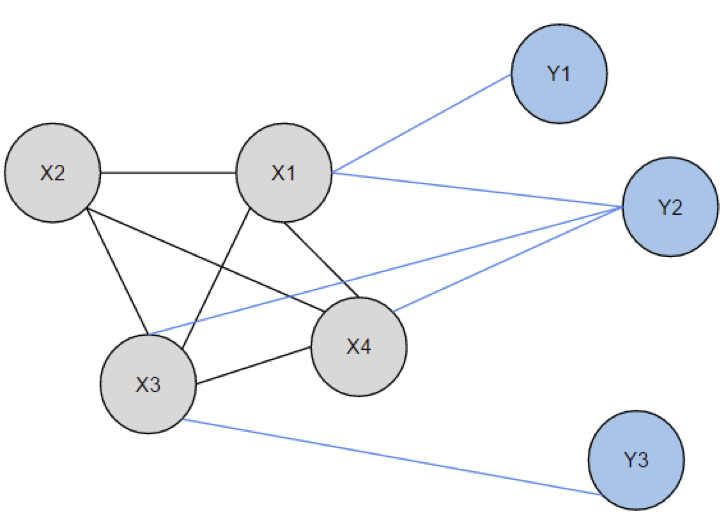
\includegraphics[width=5cm]{peripheral}
	\caption{Peripheral ingredients}
\end{figure}



There are a two primary schools of thought when designing an appropriate algorithm for recipe recommendation - using degree centrality measures, versus using pointwise mutual information (PMI). Here we enumerate in detail the algorithms.

\begin{enumerate}
	\item Degree Centrality (Fig. 1). This algorithm was the first variant that we attempted on ingredient recommendation. 


\end{enumerate}

  \begin{algorithm}
   \caption{Degree Centrality algorithm}
    \begin{algorithmic}[1]
      \Function{naive}{$recipeID$}
      	\State Let $recipe$ = recipe with ID $recipeID$
        \State Let $top10$ = ten ingredients with highest weighted number of connections
        \State Let d = dictionary to contain all ingredients and their compatibility score
        \For{$i$ in ingredients of $recipe$}
        	\If {$i$ in graph and $i$ not in $top10$}
        		\For{peripheral ingredient $k$}
        			\State{$d[k] = d[k] + \min(\frac{w(i,k)}{degree(i)},\frac{w(i,k)}{degree(k)})$}
        		\EndFor
        	\EndIf
        \EndFor
        \Return 10 ingredients from $d$ with highest compatibility score
       \EndFunction

\end{algorithmic}
\end{algorithm}


\section{Web Design}

Web design was done using a combination of HTML, CSS, JavaScript, and Python. HTML was used to create the content for display on the page, and CSS was used to style this content. JavaScript was also used for animations and general User Interface tweaks to make browsing the site intuitive and smooth. Finally, Python was utilized as an interface between the back-end and the front-end. Through the usage of Python's Flask framework, it was possible to integrate the back-end algorithms with displaying the relevant computed information on the front-end. In other words, our module app.py imported modules from the back-end, while also using this information to fill in the HTML templates based on search queries, etc. given by a user in the front end. %Thus, our architecture can be modeled in the following way:

The primary focus on the front end was to develop a site that is intuitive and self-explanatory, while also featuring only the information that is needed the most. Thus, the landing page has the following design:

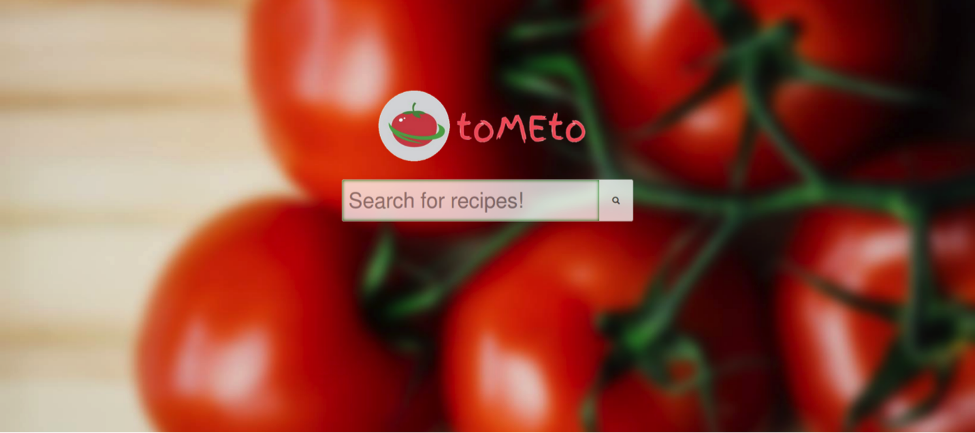
\includegraphics[scale=0.5]{p1.png}

Upon searching for a recipe, a loading bar appears, and once recipe information ins obtained, tiles fade in. These tiles offer an image of the recipe to be prepared, with the recipe title overlaid on top. This can be seen below:

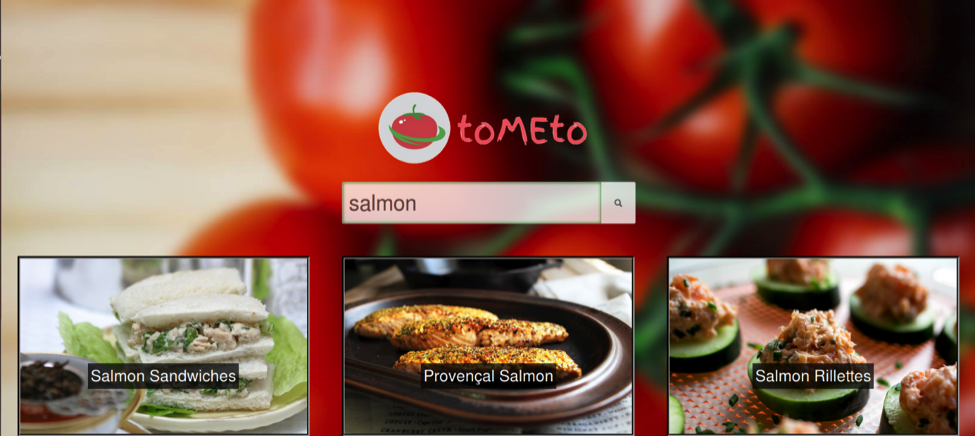
\includegraphics[scale=0.5]{p2.png}

Upon clicking a recipe, a modal popup appears, which lists both the recipe itself as well as toMEto's recommended ingredients, as can be seen in the below image:

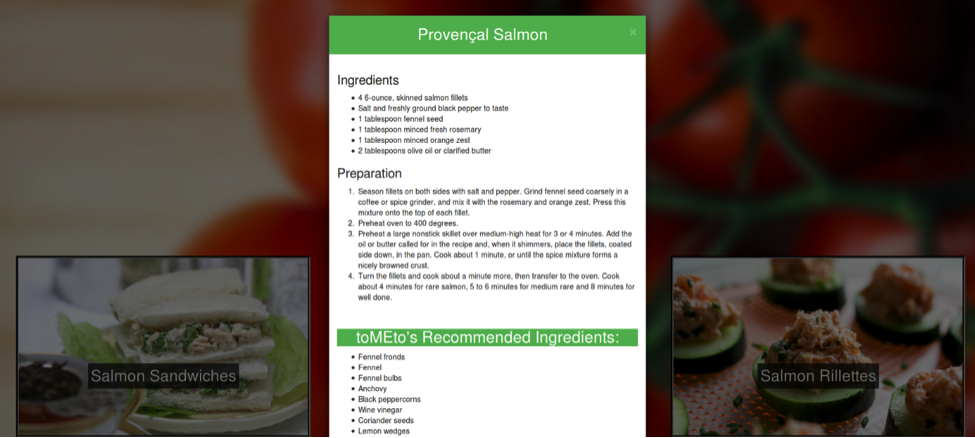
\includegraphics[scale=0.5]{p3.png}

Much of the front-end was designed to be easily updated and maintained, and thus small UI tweaks, such as background images, color schemes, etc. are easily changeable by editing the HTML and/or CSS files. The front-end utilizes mainly three different HTML templates:\begin{itemize}
\item simplesearch.html 
\item simplesearch\_searched.html 
\item no\_results.html
\end{itemize}

simplesearch.html is simply the html for the landing page, before any queries are entered. Then, once a search query is entered, app.py directs this information to the backend, which then generates information which is supplied to the simplesearch\_searched.html template. The user is also redirected to this template, which includes the tiles, modal popup information, etc. Furthermore, if a search is entered into simplesearch\_searched.html, this also refreshes the simplesearch\_searched.html template, utilizing the new information. Finally, no\_results.html is used as a template to be redirected to when the query entered into simplesearch.html or simplesearch\_searched.html does not contain any results. As a note, a user will be redirected to simplesearch.html upon clicking the toMEto logo.

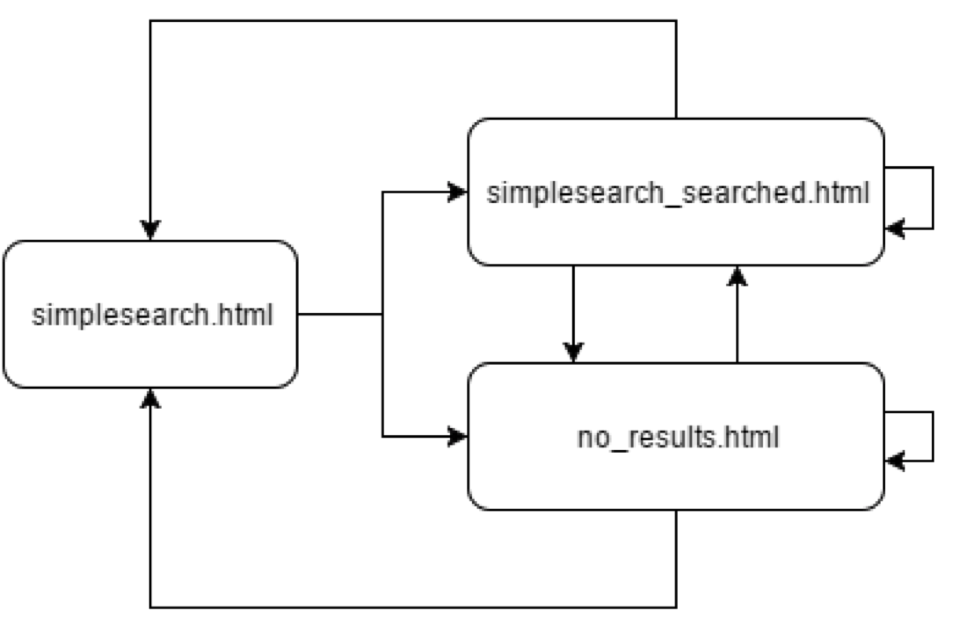
\includegraphics[scale=0.5]{p4.png}


\section{Performance}

Lorem ipsum dolor sit amet, consectetur adipiscing elit, sed do eiusmod tempor incididunt ut labore et dolore magna aliqua. Ut enim ad minim veniam, quis nostrud exercitation ullamco laboris nisi ut aliquip ex ea commodo consequat. Duis aute irure dolor in reprehenderit in voluptate velit esse cillum dolore eu fugiat nulla pariatur. Excepteur sint occaecat cupidatat non proident, sunt in culpa qui officia deserunt mollit anim id est laborum.


\section{Discussion}

Lorem ipsum dolor sit amet, consectetur adipiscing elit, sed do eiusmod tempor incididunt ut labore et dolore magna aliqua. Ut enim ad minim veniam, quis nostrud exercitation ullamco laboris nisi ut aliquip ex ea commodo consequat. Duis aute irure dolor in reprehenderit in voluptate velit esse cillum dolore eu fugiat nulla pariatur. Excepteur sint occaecat cupidatat non proident, sunt in culpa qui officia deserunt mollit anim id est laborum.



\section{Conclusions and Future Work}

Lorem ipsum dolor sit amet, consectetur adipiscing elit, sed do eiusmod tempor incididunt ut labore et dolore magna aliqua. Ut enim ad minim veniam, quis nostrud exercitation ullamco laboris nisi ut aliquip ex ea commodo consequat. Duis aute irure dolor in reprehenderit in voluptate velit esse cillum dolore eu fugiat nulla pariatur. Excepteur sint occaecat cupidatat non proident, sunt in culpa qui officia deserunt mollit anim id est laborum.


%%%%%%%%%%%%%%%%%%%%%%%%%%%%%%%%%%%
%%%% Compiling Instructions %%%%%%%
% pdflatex report.tex
% bibtex report
% pdflatex report.tex
% 
% You have to compile twice to get the references to show up


\bibliographystyle{abbrv}
\bibliography{report}

%\balancecolumns 

\end{document}

\title{CS 145 Project Plan - ToMEto}
\author{Jonathan Joo, Matthew Jin, Boyu (Charlie) Tong, Albert Ge}
\chead{%
  {\vbox{%
      \vspace{2mm}
      \large
      Networks: Structure Economics \hfill
      Caltech CMS/CS/EE 145 \hfill \\[1pt]
      CS 145 Project Plan - ToMEto \hfill
      \date{\today} \\
    }
  }
}

\linespread{1.5}


\begin{document}
\maketitle

\section{Motivation}
\subsection*{ToMEto: put the ``me'' in tomato!!}

Food is a tasty business. But it's also a difficult business. Because of the subjective nature of foods and taste, there is no good way to determine which foods go well together, and if there's any guarantee at all if a recipe that SOUNDS good will actually taste good. We've also all been in a situation where we have a bunch of random ingredients lying around, but no good idea as to which ones would work together in a recipe. Or maybe you're getting bored of a recipe you've done hundreds of times before, and you want to find an ingredient that will spice it up a little bit, but not too much that it changes the core flavor of the meal. For all of these kitchen complications, we are fortunate to have thousands upon thousands of recipes available online, most of which are tried-and-true. But the problem is, it's impossible to read through all of them to figure out what works best given your situation. Thus, we figured we would take these recipes and create a graph/database with them, and then utilize this large database of knowledge to allow for improved cooking experiences.

Past research has been done regarding food combinations, using a database of recipes. Thus, clear results exist that using such types of networks to come up with food pairing suggestions (food complements) or food substitutions is viable.\footnote{See \texttt{http://arxiv.org/pdf/1111.3919.pdf}} Furthermore, various research into these fields have yielded graph visualizations which offer the benefit of being able to see which foods are more often closely used with other foods. However, there is no easy way to use these graph visualizations to give a dynamic, helpful view on the viability of certain food pairings in a real-world context. For example, the graph in \texttt{http://www.nature.com/articles/srep00196}  does not actually do much as far as creating new or improved recipes, but simply is a network of various foods with related flavors. Our goal is to use this knowledge of past recipes to actually create suggestions upon user input, thus allowing for customized, tailored food experiences. Thus, we are motivated to take the successes of past research, and create an application that will offer dynamic feedback as to the viability of food parings, and perhaps even offer good additions to a current list of available ingredients. 



\section{Resources}

\begin{itemize}
\item Recipe recommendation using ingredient networks: \texttt{http://arxiv.org/pdf/1111.3919.pdf}
\item Flavor networks and principles of food pairing: \texttt{http://www.nature.com/articles/srep00196}
\item Data set: \texttt{http://cooking.nytimes.com/} (aggregated ratings and nutrional information!)
\item Possible (larger) data set: \texttt{allrecipes.com}
\end{itemize}

``Our experiments reveal that recipe ratings can be well predicted by features derived from combinations of ingredient networks and nutrition information (with accuracy .792), while most of the prediction power comes from the ingredient networks (84\%).''

We plan on reproducing the results of the above paper and transforming it into a web app and database. The main finding of the paper is that, using ingredient networks, the success and popularity of a recipe can be predicted with better accuracy, as opposed to simple human intuition and some naive methods. 
Thus we intend on converting these results in producing an application that will provide feedback to the user given an input of a list of ingredients, determining whether the said ingredients can be incorporated together to produce a satisfactory meal. 
This will require constructing a network structure based on the recipe dataset, experimenting with various network algorithms to optimize our recommendations or ratings, and improving the quality of feedback or recommendations (perhaps by suggesting alternative ingredients or substitutions).

First, to obtain the proper dataset, we plan on either web-scraping a popular recipe website (such as allrecipes.com or cooking.nytimes.com), or by utilizing an API (such as \texttt{Food2Fork.com}). The data collection step can be implemented in Python, and the results stored in a MySQL database. Next, to conduct analysis, we will use existing graph-building libraries (such as networkx in Python) to better understand the graph's structure. Finally, we intend to employ web development languages (HTML/CSS/Javascript) to present a front-end interface for communicating with users.



We also intend on implementing some other features, time permitting. Different regions have different tastes in food, and consequently different recipes. Trying to factor in user preferences, perhaps using a broad classification of ethnicity, into our recommendation system would be a natural extension. To do this, it is important to choose recipe datasets that are well tagged, or implement a learning system to classify them accordingly. Another possible extension is to have a more interactive recommendation system. If an ingredient likely does not fit in well, our app could suggest removing it. On the other hand, it could suggest an ingredient that would fit well, or perhaps even revolutionary new ingredients from other cuisines, creating a fusion dish. This extension is quite a bit more ambitious, and would also require some culinary skills and hands-on experimenting.



\section{Timeline}

\textbf{Week 1 - Understand the environment} \\
Flesh out project goals, investigate APIs, etc. Record all recipe sites and how easy it would be to get data off of each. Compare skillsets and divide labor according to strengths of each group member.

\textbf{Week 2 - Data farming} \\
Connect with APIs and write crawlers/scrapers if necessary. Begin scraping and pulling raw recipe data. Take care not to get throttled or banned. Store recipe data locally in a database.

\textbf{Week 3 - Data compiling} \\
Continue pulling raw recipe data. Construct a graph with the data, weighting edges based on prevalence among recipes. Investigate different data processing techniques, pruning edges, etc. Figure out which results in the most relevant and useful graph.

\textbf{Week 4 - Data analyzing} \\
Analyze clustering and visualization techniques. Investigate the best way to cluster complementary ingredients and research a way to visualize the clusters (third party libraries or other). 

{\em \textbf{* Milestone 1:}} Have a graph visualization of the pulled data. 

\textbf{Week 5 - Web framework} \\
Write a web framework. Two components: bring up a backend service for hosting the data, and a front end web application that displays information to the user. At this point, there's only basic functionality: user can view ingredients list.

{\em \textbf{* Milestone 2:}} Test users can connect to the app and view the ingredients list.

\textbf{Week 6 - Feature: Combination rater} \\
Given a list of ingredients, calculates how well they all work together. Try out a bunch of different metrics to determine which one works best (depends on graph implementation). 

\textbf{Week 7 - Feature: Supplementary ingredients} \\
User can input a list of ingredients, and the server will find an ingredient that works well with everything else (or a list of top 5 ingredients that are complementary, as well as a metric/score for each). 

\textbf{Week 8 - Feature: Separate by cuisines} \\
Recipe data is first parsed and grouped by cuisine (Indian, Italian, Chinese, etc.). Use machine learning to categorize unknown recipes. Users can restrict results to contain only certain ingredients.

\textbf{Week 9 - Polish and push} \\
Polish application. Make GUI aesthetically pleasing. Fix bugs on server and frontend application. Improvements on algorithms used for clustering, categorizing cuisines, etc. Publicly release the application, having friends and other people at school test out the application.

{\em \textbf{* Milestone 3:}} Public launch, users now can start using the app and the implemented features.

\textbf{Week 10+ - Further expansion} \\
Further features and improvements: dynamic graph structure (user feedback on ingredient combinations), fusion cuisine (combine two cuisines and see what kind of flavors emerge). 



\end{document}
